\chapter{Sortieren und Suchen}
\section{Vergleichsbaummodell}
Das Vergleichsbaummodell modelliert Algorithmen, die nur auf Vergleichen zwischen Elementen der Eingabefolge beruhen. $\mathcal{U}$ sei ein Universum auf dem eine lineare Ordnung $\le$ definiert ist. Die Eingabefolge ist definiert als $a_1, \ldots, a_n \in \mathcal{U}$.

\begin{figure}[htb]
  \centering
  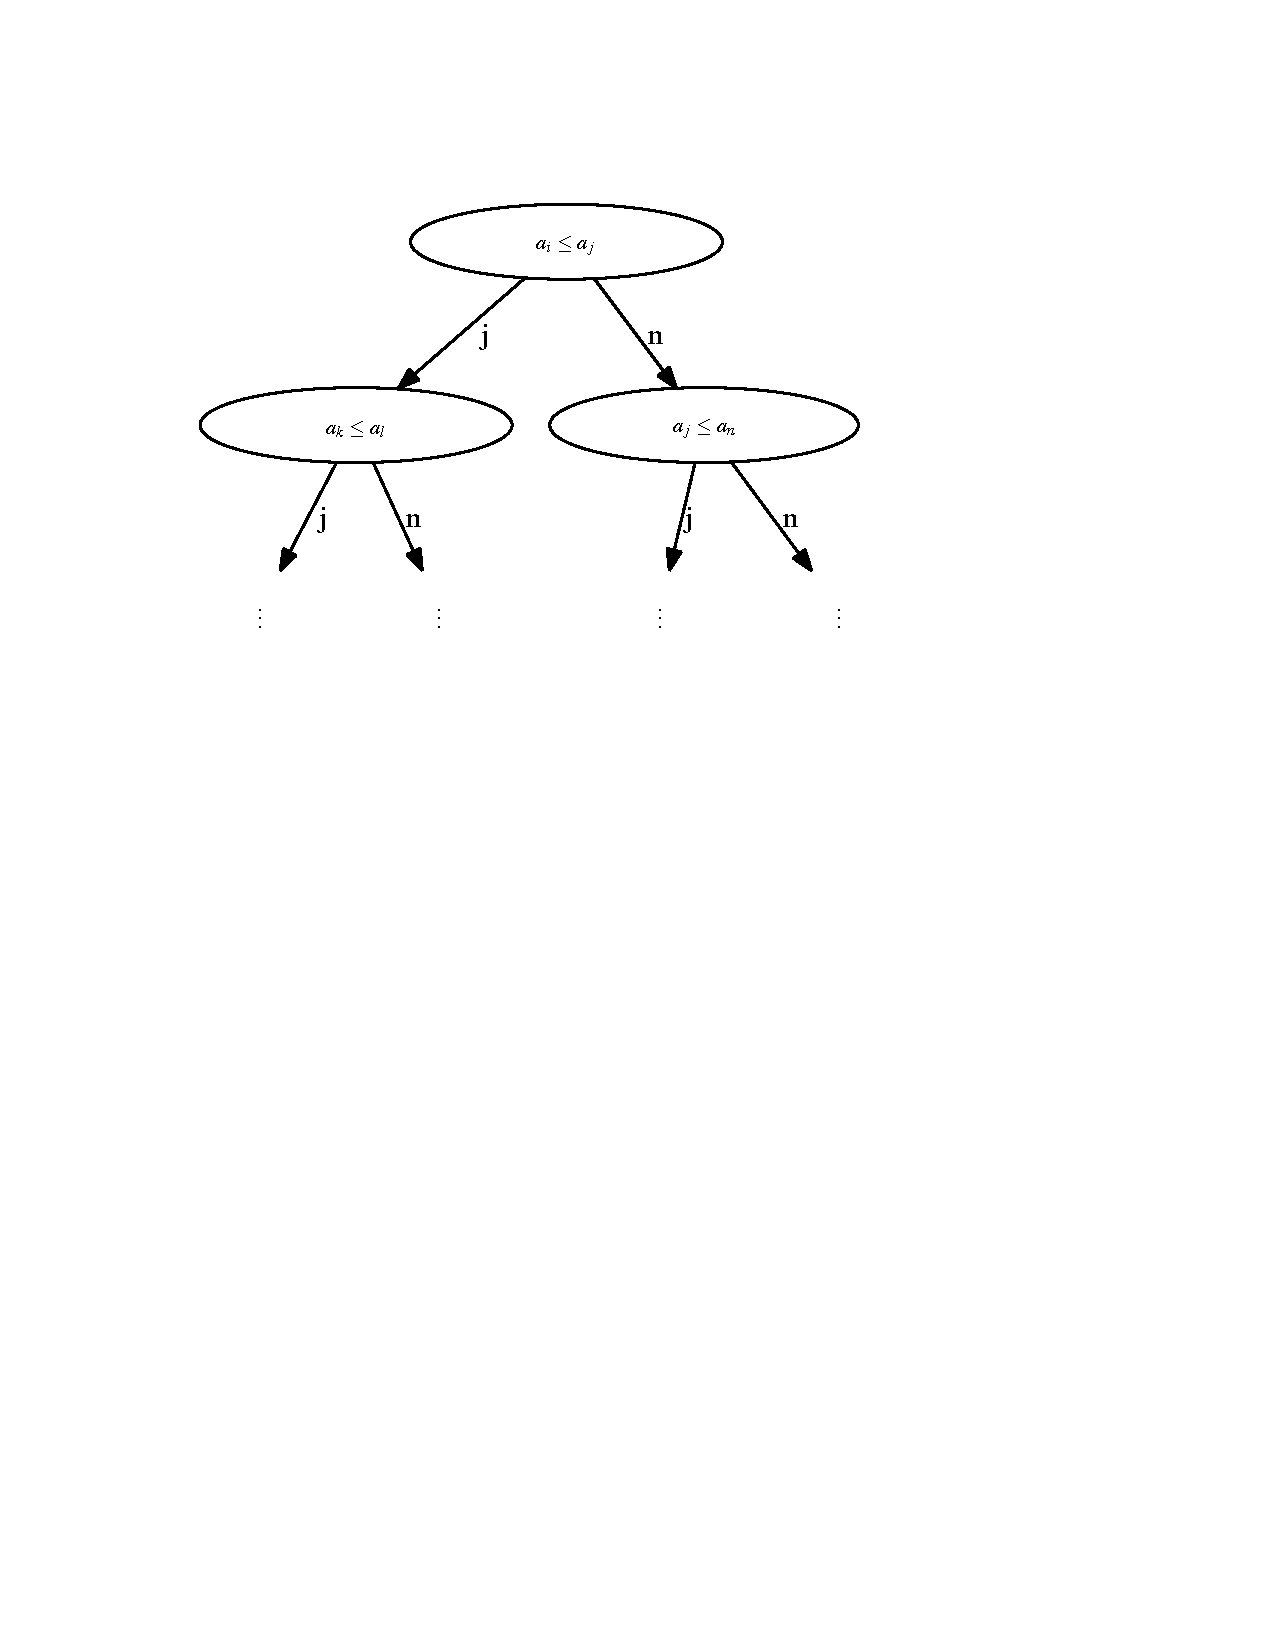
\includegraphics[scale=.75]{kap2graph1.pdf}
  \caption{Vergleichsbaum für einen Algorithmus und eine Eingabe $a_1, \ldots, a_n$}
\end{figure}

Die Algorithmen \ref{Bogosort} bis \ref{Alter-Mann} lassen sich für feste $n$ als Vergleichsbäume darstellen.

\begin{figure}[htb]
  \centering
  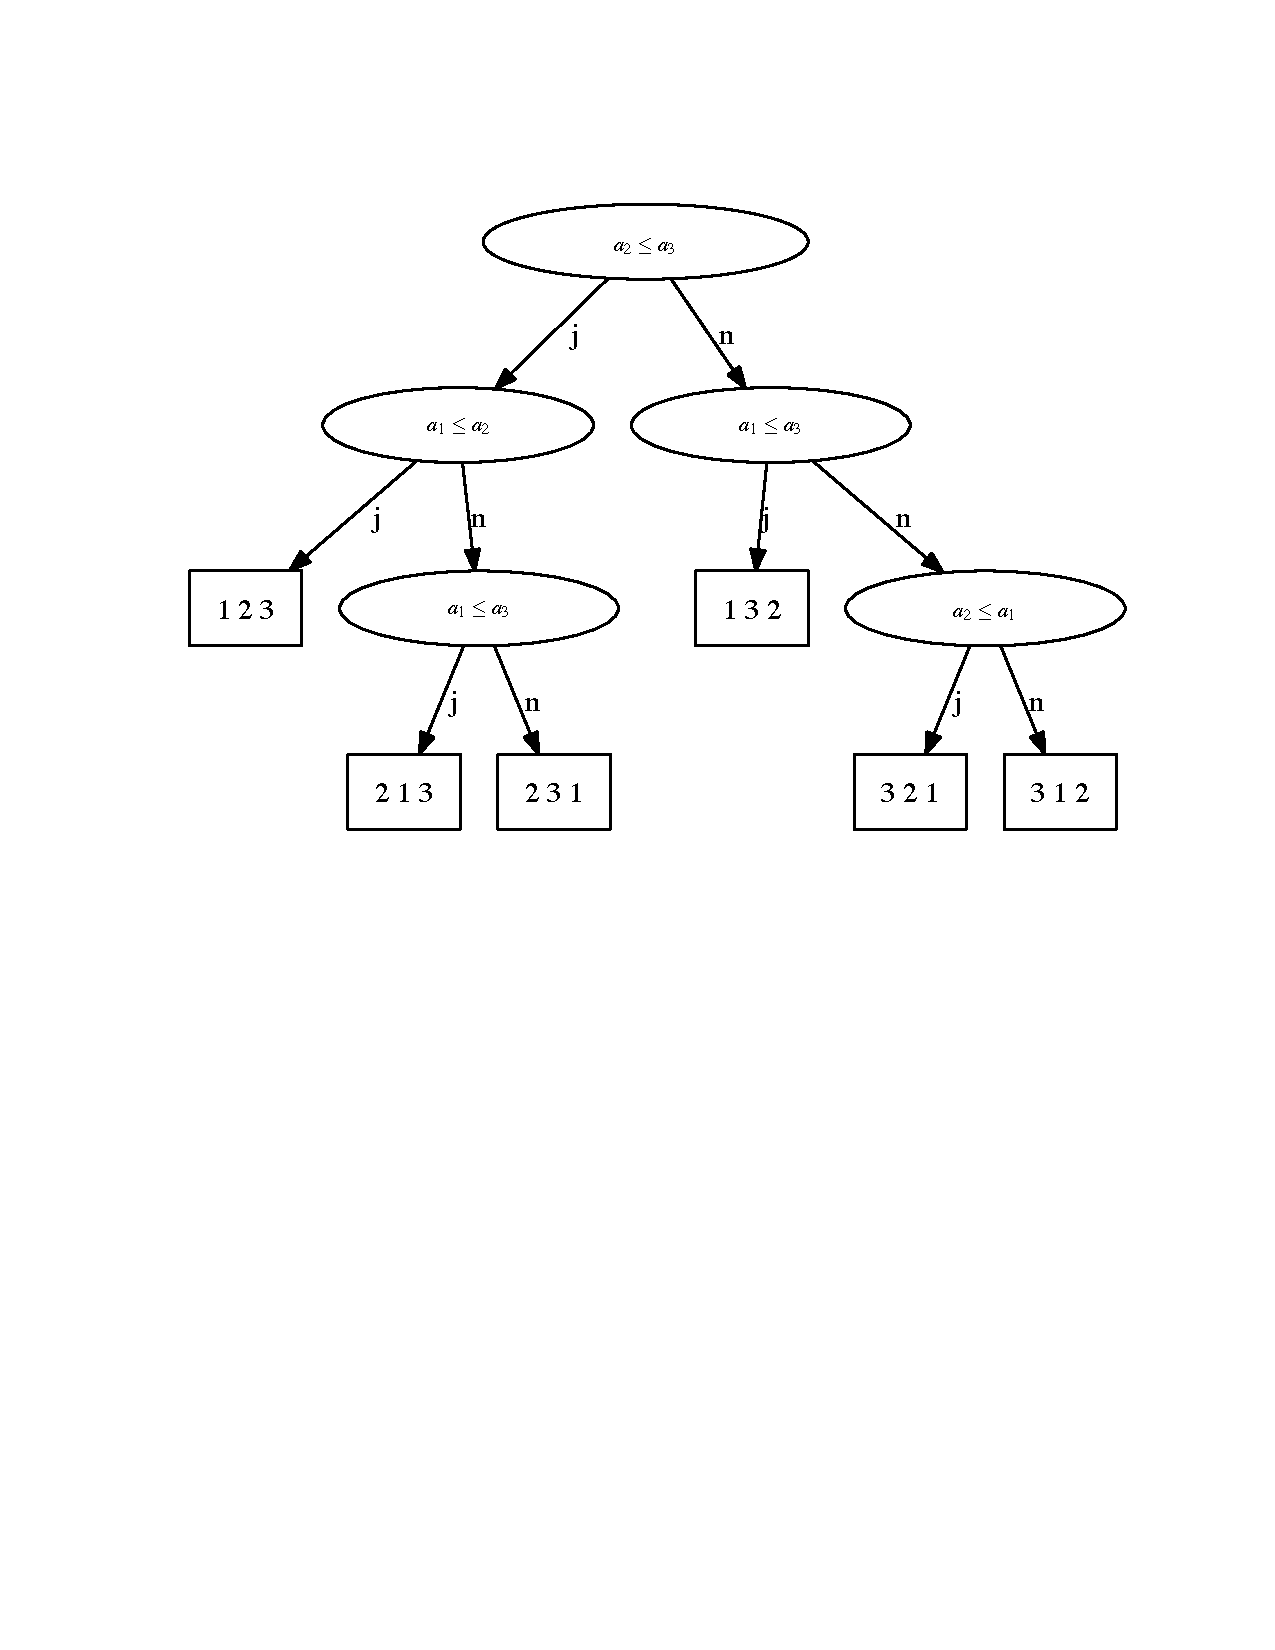
\includegraphics[scale=.75]{kap2graph2.pdf}
  \caption{Vergleichsbaum für Mergesort und die Eingabe $a_1, a_2, a_3$}
\end{figure}

In den Blättern des Vergleichbaums finden wir das Ergebnis des Algorithmus. Für vergleichsbasiertes Sortieren könnnen wir durch den Vergleichsbaum eine untere Schranke zeigen.

\subsection{Untere Schranke für vergleichsbasierte Sortieren}
Allgemeine Sortierverfahren funktionieren auf beliebigen, linear geordnetem Universum. Für allgemeine Sortierverfahren kann man eine untere Schranke zeigen. Für spezielle Universen (z.B. $\lbrace 0, 1 \rbrace$) lassen sich schnellere Sortierverfahren finden.

Eine untere Schranke ist eine Aussage der Form: für jede Eingabe der Länge $n$ braucht man mindestens $T(n)$ Vergleiche. Eine untere Schranke kann auch eine Aussage der Form sein: es gibt eine Eingabe der Länge $n$ zu deren Sortierung man mindestens $T(n)$ Vergleiche braucht. Anstatt auf Vergleichen können sich die Aussagen natürlich auch auch auf Laufzeit, Speicher oder der Gleichen beziehen.

Ein Vergleichsbaum zum Sortieren einer Folge der Länge $n$ muss mindestens $n!$ Blätter haben, da $n!$ der Anzahl aller möglichen Permutation einer Folge der Länge $n$ entspricht. Ein Vergleichsbaum ist binär, das heißt bei Höhe $h$ hat er maximal $2^h$ Blätter. Die Höhe entspricht einem Lauf durch den Vergleichsbaum von oben nach unten mit einer maximal langen Folge von Vergleichen. Die Anzahl der Blätter lässt sich also durch $2^h \ge \text{Anzahl der Blätter} \ge n!$ abschätzen, mit $h \ge \log n!$.
Wir können $n!$ wie folgt abschätzen:
\[n! = 1 \cdot 2 \cdot \ldots \cdot \frac{n}{2} \cdot \underbrace{\left(\frac{n}{2}+1\right) \cdot \ldots \cdot n}_{\ge \frac{n}{2}} \ge \frac{n}{2}^{\frac{n}{2}}\]
Also gilt $\log n^n \ge \log n! \ge \log \frac{n}{2}^{\frac{n}{2}}$. Genauer lässt sich $n!$ noch durch die Stirlingsche Formel abschätzen: $n! = \sqrt{2 \pi n} \left(\frac{n}{e}\right)^n e^{\frac{\Theta}{12n}}$ wobei $0<\Theta<1$.

Wegen der Logarithmengesetze  ist $\log \frac{n}{2}^{\frac{n}{2}} = \frac{n}{2} (\log n-1)$. Mit den Logarithmengesetzen und der Stirlingschen Formel können wir $\log n!$ wie folgt abschätzen.

\begin{align*}
\log n! &= \log \left(\sqrt{2 \pi n} \left(\frac{n}{e}\right)^n e^{\frac{\Theta}{12n}}\right) \\
          &= \frac{1}{2} \log n + \frac{1}{2} \log 2 \pi + n (\log n - \log e) + \frac{\Theta}{12n} \log e\\
%          &= \frac{1}{2} \log n + n\left(\log n - \log e \right) + \log e \frac{\Theta}{12n} + \frac{1}{2}\log 2 \pi \\
          &= n \log n - n \log e + \frac{1}{2} \log n + \frac{1}{2} \log 2 \pi +  o(1)
\end{align*}

$\lim\limits_{n \rightarrow \infty}{o(1)} = 0$, also ist $h \ge n \log{n} - \mathcal{O}(n)$ für hinreichend große $n$.

\begin{Satz}[Untere Schranke für vergleichsbasiertes Sortieren]
\hspace{\parindent}Im Vergleichsbaummodell braucht jeder Algorithmus zum Sortieren einer Folge der Länge $n$ im schlechtesten Fall mindestens $n \log{n} -\mathcal{O}(n)$ Vergleiche.
\end{Satz}

Das heißt man kann nicht schneller sortieren als $n \log{n} -\mathcal{O}(n)$. Für spezielle Universen kann man das wie gesagt schlagen, im Allgemeinen Fall aber nicht.

%\section{Berechnungsbaummodell}
Algebraische Berechnungsbäume sind ein erweitertes Modell der Vergleichsbäume. Vergleichsbäume werden dabei um Rechnungen erweitert, so dass in algebraischen Berechnungsbäumen auch $+, -, *, /$ verwendet werden können.

Auch mit diesem Modell lässt sich $\Omega(n \log n)$ als untere Schranke für allgemeine Sortierverfahren zeigen.

\subsection{Weitere untere Schranken}
\begin{Exk}[Landau-Notation]
\hspace{\parindent}Landau-Symbole werden verwendet, um das asymptotische Verhalten von Funktionen und Folgen zu beschreiben.

\begin{center}
\begin{tabular}{lp{14em}c}
Notation & Bedeutung & math. Definition \\\hline\hline
$f \in \mathcal{O}(g)$ & obere Schranke: $f$ wächst nicht wesentlich schneller als $g$ & $0 \le \limsup\limits_{x \to a} \left|\frac{f(x)}{g(x)}\right| < \infty$ \\
$f \in o(g)$ &$f$ wächst langsamer als $g$ (asymptotisch vernachlässigbar)&$\lim\limits_{x \to a} \left|\frac{f(x)}{g(x)}\right| = 0$\\
$f \in \Omega(g)$ &$f$ wächst nicht wesentlich langsamer als $g$ (untere Schranke)&$0 < \liminf\limits_{x \to a} \left|\frac{f(x)}{g(x)}\right| \le \infty$\\
$f \in \omega(g)$ &$f$ wächst schneller als $g$ ($g \in o(f)$)&$\lim\limits_{x \to a} \left|\frac{f(x)}{g(x)}\right| = \infty$\\
$f \in \Theta(g)$ &$f$ und $g$ wachsen gleich schnell ($f \in \mathcal{O}(g)$ und $g \in \mathcal{O}(f)$)&$0 < \liminf\limits_{x \to a} \left|\frac{f(x)}{g(x)}\right| \le \limsup\limits_{x \to a} \left|\frac{f(x)}{g(x)}\right|< \infty$\\\hline\hline
\end{tabular}
\end{center}
\end{Exk}

$\Omega(n \log n)$ gilt nicht nur für allgemeine Sortiverfahren als untere Schranke. Ein anderes Problem mit der selben unteren Schranke ist das Problem der \textit{Mengengleichheit}. Gegeben sind zwei Mengen über einem Universum: $S, T \subseteq \mathcal{U}$. Gefragt ist, ob $S$ und $T$ gleich sind, also $S=T$? Entscheiden lässt es sich in $n \log n$, in dem man beide Mengen sortiert und anschließend in linearer Zeit vergleicht.

Ein weiteres Problem der Art ist das Problem der \textit{element uniqueness}. Gegeben ist eine Folge $S \subseteq \mathcal{U}$ der Länge $n$ mit den Elementen $a_1, \ldots a_n$. Gibt es $i,j$ mit $i\neq j$, so dass gilt $a_i = a_j$?

Es gibt nicht viele Probleme mit bekannten unteren Schranken. Interessant ist, dass es noch andere Wege gibt die untere Schranke für allgemeine Sortierverfahren zu zeigen, als über das Vergleichsbaummodell.

Wir wollen hier aber noch ein Problem mit einer anderen unteren Schranke betrachten: \textit{Finden des Maximums}. Das triviale Vorgehen ist sicherlich das erste Element mit dem zweiten zu vergleichen und sich das Größere der beiden zu merken. Alle weiteren Elemente werden dann mit dem bis dahin gefundenen Maximum verglichen, so dass man auf eine Laufzeit von $n-1$ kommt. Warum geht es aber nicht schneller als mit $n-1$ Vergleichen? Jedes Element, das nicht als Maximum deklariert wird, muss in einem Vergleich unterlegen gewesen sein: Es gibt im allgemeinen Fall keine Möglichkeit zu erkennen, dass ein Element nicht das Maximum ist, ohne es zu Vergleichen. Jedes Element muss also mind. einmal verglichen worden sein, daher braucht man mindestens $n-1$ Vergleiche.

\section{Sortieren in linearer Zeit}
Sortieren in linearer Zeit lässt sich weder im Vergleichsbaummodell realisieren noch für den allgemeinen Fall. Wir wollen hier Algorithmen betrachten, die spezielle Universen in linearer Zeit sortieren. Betrachten wir zunächst das Universum $\mathcal{U} = \lbrace 0, 1 \rbrace$. Hier kann man in $\mathcal{O}(n)$ mit zwei Zählern sortieren, indem man erst alle $0$- und dann alle $1$-Elemente zählt und anschließend die richtige Anzahl in der richtigen Reihenfolge ausgibt. Verallgemeinert auf beliebige endliche Universen $\mathcal{U} = \lbrace c_1, \ldots, c_k\rbrace$ braucht man $k = |\mathcal{U}|$ Zähler.

\textit{Bucketsort} ist eine Verallgemeinerung des Sortierens in linearer Zeit. Allen zu sortierenden Elemente muss dazu ein Wert zugewiesen werden können. Die Eingabe kann dann als Intervall angesehen werden, dass in gleichgroße Teilintervalle aufgeteilt werden kann, in sogenannte "`Buckets"'. In diese Buckets werden dann die Elemente einsortiert. Wenn die Elemente gleichverteilt sind und die Anzahl der Buckets der Anzahl der Elemente entspricht (ein Element pro Bucket), so arbeitet Bucketsort in linearer Zeit. Andernfalls müssen die Buckets intern sortiert und dann konkateniert ausgegeben werden. Bucketsort hat dann die Laufzeit des Algorithmus, der zum Sortieren der Buckets genutzt wird. Diese Verfahren ist zum Beispiel gut geeignet, um Briefe anhand von Postleitzahlen zu sortieren.

\textit{Radixsort} ist ein Algorithmus zum Sortieren von Wörtern $\in \Sigma^*$ mit $\Sigma$ endliches Alphabet. Es basiert auf Bucketsort. Das Ziel ist es die eingegebenen Wörter in lexikographische Ordnung zu bringen. Dabei hat jeder Buchstabe in einem Wort ein unterschiedliches Gewicht, je nach seiner Position (größtes Gewicht hat der erste Buchstabe, kleinstes Gewicht der letzte). Radixsort sortiert die Wörter wie folgt: zu erst werden die Wörter anhand ihres letzten Buchstaben sortiert. In weiteren Läufen werden die Buchstaben von hinten nach vorne verglichen und die Reihenfolge der Wörter nur verändert, wenn die betrachteten Buchstaben nicht in lexikographischer Ordnung stehen. Ein Beispiel ist in Abb. \ref{radixBsp} zu sehen.

\begin{figure}[hbt]
\centering
\begin{tabular}{ccccccc}
Mon & \multirow{4}{*}{$\xrightarrow{\stackrel{\text{\small letzer}}{\text{\small Buchstabe}}}$} & Die & \multirow{4}{*}{$\xrightarrow{\stackrel{\text{\small vorletzer}}{\text{\small Buchstabe}}}$}& Die & \multirow{4}{*}{$\xrightarrow{\stackrel{\text{\small erster}}{\text{\small Buchstabe}}}$} & Die \\
Die &  & Mon & & Mit & & Don \\
Mit &  & Don & & Mon & & Mit \\
Don &  & Mit & & Don & & Mon \\
\end{tabular}
\caption{Radixsort auf den Wörtern Mon, Die, Mit, Don.}\label{radixBsp}
\end{figure}


Radixsort braucht $\mathcal{O}(n)$ Zeit, wobei $n$ der Gesamtzahl der Buchstaben aller Wörter entspricht.

\section{Das Auswahlproblem (selection, order statistics, Select)}
Betrachten wir das Auswahlproblem: Als Eingabe bekommen wir eine Folge $S$ von $n$ Elementen aus dem Universum $(\mathcal{U}, \le)$ und die Zahl $k$ mit $1 \le k \le n$. Gesucht ist das k-t-kleinste Element von $S$, also das Elemente, das an Stelle $k$ der Folge $S$ steht, wenn sie aufsteigend sortiert ist. Dieser Ansatz --~sortieren der Folge und abzählen der Stelle $k$~-- liefert bereit einen Algorithmus, mit Laufzeit $\mathcal{O}(n \log n)$. Geht das noch schneller?

\subsection{Randomisiertes Select}
\begin{Alg}[SELECT(k, S)]
	\begin{enumerate}
	  \item Falls $|S|=1$ (also $S = \lbrace a \rbrace$), return $a$, sonst:
	  \item Wähle zufällig ein Element $a \in S$.
	  \item Spalte $S$ in drei Teilfolgen: $S_1 = \lbrace\text{Elemente} < a\rbrace$, $S_2 = \lbrace\text{Elemente} = a\rbrace$ und $S_3 = \lbrace\text{Elemente} > a\rbrace$.
	  \item Falls $k \leq |S_1|$, dann return \textsc{Select}$(k, S_1)$.
	  \item Falls $k \leq |S_1| + |S_2|$ dann return $a$.
	  \item Sonst return \textsc{Select}$(k-|S_1| - |S_2|, S_3)$.
	\end{enumerate}
\end{Alg}

Dieser Algorithmus ist mit Quicksort vergleichbar. Er hat die gleiche Schwäche: Wenn man $a$ ungünstig wählt, ist die Laufzeit im schlechtesten Fall $\Theta(n^2)$. Doch wie ist die erwartete Laufzeit, also die Laufzeit im Mittel?

Der Rekursionsanker ist einfach zu finden: $T(1) = b$, wobei $b$ konstant ist. Stellen wir die Rekursionsgleichung für $T(n)$ auf: Sei $a$ das $i$-t-kleinste Element (also das Element an Stelle $i$, falls die Folge aufsteigend sortiert ist). Dann ist $S_1 = \{ a_1, \ldots, a_{i-1}\}$, $S_2 = \{ a_i \}$ und $S_3 = \{ a_{i+1}, \ldots , a_n \}$ . Jedes $i \in \{1, \ldots, n\}$ hat eine Wahrscheinlichkeit von $\frac{1}{n}$. Falls $i<k$, so liegt das gesuchte Element in $S_3$. Wir starten also eine rekursive Suche in $S_3$, einer Teilfolge der Größe $n-i$. Angenommen $i > k$, so liegt das gesuchte Element in $S_1$, also in einer Teilfolge der Größe $i-1$. Der Fall $i=k$ ist durch $T(1)$ bereits abgedeckt. Die Rekursionsgleichung lässt sich daher wie folgt aufstellen:

\[ T(n) = \frac{1}{n} \left(\vphantom{\sum_{i=1}^{k-1}}\right. \underbrace{\sum_{i=1}^{k-1} T(n-i)}_{\text{rek. Aufruf für} S_3} + \underbrace{\sum_{i=k+1}^{n} T(i-1)}_{\text{rek. Aufruf für} S_1} \left.\vphantom{\sum_{i=1}^{k-1}}\right) + \underbrace{c \cdot n}_{\text{fürs Aufteilen}}\]

Betrachten wir kurz die beiden Summen in dieser Gleichung. In der ersten Summe verläuft $i$ von $1$ bis $k-1$. Es wird also summiert über $T(n-1) + T(n-2) + \ldots + T(n-k+1)$. In der zweiten Summe verläuft $i$ von $k+1$ bis $n$. Es wird also summiert über $T(k) + \ldots + T(n-2) + T(n-1)$.

\begin{figure}[hbt]
  \centering
  \includegraphics{kap2strahl1}
  \caption{Angenommen $k \leq \frac{n}{2}$. Der mittlere Bereich visualisiert die erste, der untere die zweite Summe. Der blaue gepunktete Bereich entspricht: $k \ldots \frac{n}{2}$, der grüne gestrichelte größere Bereich $\frac{n}{2} \ldots (n-k+1)$.}
  \label{kap2strahl1}
\end{figure}

Angenommen $k \leq \frac{n}{2}$. Wir können $k \ldots \frac{n}{2}$ durch $\frac{n}{2} \ldots n-k+1$ ersetzen, da $T$ monoton steigend und somit der ersetzte Bereich kleiner ist, als der ersetzende Bereich. In Abbildung \ref{kap2strahl1} wird das ganze veranschaulicht: wir ersetzen den blauen, durch den grünen Bereich. Dadurch können wir die beiden Summen zu einer zusammenfassen, und schreiben:
\[T(n) \leq \frac{2}{n} \sum_{i= \lfloor \frac{n}{2} \rfloor}^{n-1} T(i) + c \cdot n\]

Behauptung: $T(n) = \mathcal{O}(n)$. Das heißt $\exists{} d > 0 : T(n) \le d n$ für alle $n \in \mathbb{N}$. Wir wollen das durch Induktion über n beweisen.

Wir nehmen an, dass eine Konstante $d$ existiert, so dass gilt $T(n) \le d \cdot n$.
Als Induktionsanfang dient uns $n=1$. Anhand von Zeile $1$ des Algorithmus kann man sehen, dass $T(1) = b \le d$. Für ein geeignet gewähltes $d \ge b$ ist das richtig.
Es folgt der Induktionsschritt $(n-1) \rightarrow n$:

\[T(n) \le \frac{2}{n} \sum_{i= \lfloor \frac{n}{2} \rfloor}^{n-1} T(i) + cn\]
Aufgrund der Induktionsvoraussetzung können wir annehmen, dass 
\[\sum_{i= \lfloor \frac{n}{2} \rfloor}^{n-1} T(i) \le \sum_{i= \lfloor \frac{n}{2} \rfloor}^{n-1} d \cdot i\]
Daher gilt:
\[T(n) \le \frac{2d}{n} \sum_{i=\lfloor\frac{n}{2}\rfloor}^{n-1} i + cn\]
Die Summe schätzen wir mit dem Satz von Gauß ab, wobei wir aufgrund des Laufindex der Summe den zu viel berechneten Teil subtrahieren müssen.
\[ T(n) \le \frac{2d}{n} \left( \frac{n(n-1)}{2} - \frac{\lfloor \frac{n}{2} \rfloor(\lfloor \frac{n}{2} \rfloor -1)}{2} \right) + cn \qquad \lfloor \frac{n}{2} \rfloor \ge \frac{n}{2}-1 \]
Unter Berücksichtigung der Abschätzung $\lfloor \frac{n}{2} \rfloor \ge \frac{n}{2} -1$ können wir schreiben:
\begin{align*}
T(n) & \le \frac{2d}{n} \left( \frac{1}{2}n^2 - \frac{1}{2} n - \frac{(\frac{n}{2} -1) (\frac{n}{2}-2)}{2}\right) + cn\\
     & \le \frac{2d}{n} \left( \frac{3}{8} n^2 + \frac{1}{4}n -1 \right) + cn
\end{align*}
Die $-1$ können wir weg lassen, für die Ungleichung ist das unerheblich.
\begin{align*}
T(n) & \le \frac{3}{4}dn + \frac{1}{2}d + cn \\
     &  = \left( \frac{3}{4} d + c \right) n + \frac{d}{2}
\end{align*}
Gegen die $\frac{d}{2}$ können wir noch etwas machen: Die $\frac{3}{4}d$ ersetzen wir durch $0{,}8d$ und ziehen dann $0{,}05dn$ vom zweiten Summanden ab.
\[ T(n) \le (0{,}8 d + c) n + \left(\frac{1}{2} - 0{,}05 n\right) \cdot d \]
Für $n \ge 10$ nimmt $\left(\frac{1}{2} - 0{,}05 n\right) \cdot d$ einen Wert $\le 0$ an, das heißt für diese $n$ ergibt sich:
\[T(n) \le (0{,}8 d + c) n\]
Wir können nun wiederum abschätzen $0{,}8 d + c \le d$ und nach $d \le 5c$ auflösen. So erhalten wir schließlich für $n \ge 10$
\[T(n) \le dn\]

Für $n < 10$ braucht Algorithmus konstant viele Schritte: $T(n) \le e$. Wählen wir $d \ge e$ dann gilt $T(n) \le dn$ für alle $n \in \mathbb{N}$. Die Behauptung gilt also mit $d=max (b, 5c, e)$.

\begin{Satz}
\hspace{\parindent}Der Algorithmus \textsc{Select} löst das Auswahlproblem mit mittlerer Laufzeit $\mathcal{O}(n)$ für Folgen der Länge $n$.
\end{Satz}

\subsection{Deterministisches Select}
Können wir einen deterministischen Select-Algorithmus finden, mit garantierter Laufzeit von $\mathcal{O}(n)$? Wir ersetzen die ersten beiden Zeilen im Select"=Algorithmus durch folgende:

\begin{enumerate}
  \item Falls $|S| < 60$, löse das Problem "`brute force"' zum Beispiel durch sortieren und auswählen. Sonst:
  \item \begin{itemize}
    \item Teile $S$ in $\lceil \frac{n}{5} \rceil$ Teilfolgen der Länge 5
    \item bestimmte von allen Teilfolgen die "`Mediane"' (d.h. k-tes Element für $k=\lceil \frac{5}{2} \rceil$)
    \item bestimme von diesen $\lceil \frac{n}{5} \rceil$ Medianen rekursiv den Median und wähle ihn als Element $a$ aus.
  \end{itemize}
\end{enumerate}

Warum ist die Laufzeit garantiert linear? In Abbildung \ref{mediansuche} sieht man, dass durch ein klug gewähltes $a$ ein konstanter Bruchteil an Elementen wegfällt und nicht untersucht werden muss.

\begin{figure}[htb]
  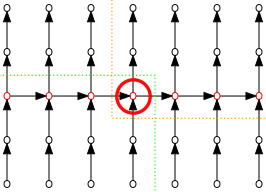
\includegraphics{kap2mediansuche}
  \centering
  \caption{Graphische Darstellung der Mediansuche: von links nach rechts sieht man die fünf\-ele\-men\-ti\-gen Teilfolgen, jeweils von oben nach unten absteigend sortiert (ein Pfeil steht für $\le$). Die roten Punkte markieren die Mediane, der rote Kreis den Median der Mediane. Die \textcolor{green}{grüne} Box markiert die Menge A, die alle Elemente enthält von denen aus es einen gerichteten Pfad zum Median der Mediane gibt. Die \textcolor{orange}{orangene} Box markiert die Menge B, die alle Elemente enthält zu denen es einen gerichteten Pfad vom Median der Mediane aus gibt. Beim Aufspalten fällt eine von beiden Mengen weg, so dass der rekursiver Aufruf höchstens die übrigen Elemente untersuchen muss.}
  \label{mediansuche}
\end{figure}

Wenn $n$ kein Vielfaches von 5 ist, können wir neben der letzten fünfelementigen Teilmenge bis zu vier weitere Elemente habe. Diese berücksichtigen wir bei der Mediansuche nicht, sie fließen einfach direkt in die Menge der Elemente ein, die später untersucht werden.

Wir wissen, dass es in Abbildung \ref{mediansuche} einen gerichteten Pfad von allen Elementen der Menge $A$ zu $a$, dem Median der Mediane gibt. Daher gilt $\forall b \in A : b \le a$. Analog können wir folgende Aussage gestalten $\forall b \in B : b \ge a$. Beim Aufspalten bezüglich $a$ fällt daher die Menge $A$ oder die Menge $B$ weg. Der rekursive Aufruf untersucht daher höchstens die restlichen Elemente. Es gibt $\frac{n}{5}$ Teilfolgen, von denen die eine Hälfte zu $A$ beiträgt, die andere Hälfte zu $B$. Jede Teilfolge hat fünf Elemente, von denen wiederum die Hälfte zu $A$ beziehungsweise zu $B$ gehört. Wir können die Größe von $A$ und $B$ somit abschätzen als $|A| \ge \lceil\frac{\lfloor\frac{n}{5}\rfloor}{2} \rceil \cdot 3 = 3 \cdot \lfloor \frac{n}{10} \rfloor \le |B|$.

Die rekursiven Aufrufe betreffen daher höchstens $|S_1|, |S_3| \le n - 3 \lfloor \frac{n}{10} \rfloor$ Elemente. Diese können wir weiter abschätzen: Es gilt $n - 3 \lfloor \frac{n}{10} \rfloor \le n - 3 (\frac{n}{10} - 1) = 0,7 n + 3 \le 0,75 n$ falls $3 \le 0,05 n$ also für hinreichend Große $n \ge 60$. Dies begründet die erste Zeile des Algorithmus, die für die ersten 60 Elemente einen Brute-Force-Ansatz wählt.

Wir erhalten folgende Rekursions(un)gleichung:
\begin{align*}
  T(n) &\le c \qquad\text{für n < 60}\\
  T(n) &\le \underbrace{T(\lfloor\frac{3}{4}n\rfloor)}_{\text{für den Rek. Aufruf}} + \underbrace{T(\lfloor \frac{n}{5} \rfloor)}_{\text{für die Mediansuche}} + \underbrace{dn}_{\text{aufteilen in } S_1, S_2, S_3} + \mathcal{O}(n)
\end{align*}
%Wir erhalten folgende Rekursions(un)gleichung:
%\begin{align*}
%  T(n) &\le c \qquad\text{für n < 60}\\
%  T(n) &\le \underbrace{T(\lfloor\frac{7}{10}n\rfloor)}_{\text{für den Rek. Aufruf}} + \underbrace{T(\lfloor \frac{n}{5} \rfloor)}_{\text{für die Mediansuche}} + \underbrace{dn}_{\text{aufteilen in } S_1, S_2, S_3}
%\end{align*}
%
%Es gilt $n - 3 \lfloor \frac{n}{10} \rfloor \le n - 3 (\lfloor \frac{n}{10} \rfloor-1) = 0,7 n + 3 \le 0,75 n$ falls $3 \le 0,05 n$ also für hinreichend Große $n \ge 60$. Dies begründet die erste Zeile des Algorithmus, die für die ersten 60 Elemente einen Brute-Force-Ansatz wählt. Für hinreichend große $n$ können wir abschätzen $\frac{n}{5} \le \frac{n}{5} +1 \le \lfloor 0,25 n \rfloor$. Wir können also schreiben:
%\[ T(n) \le T(\lfloor\frac{3}{4}n\rfloor) + T(\lfloor \frac{n}{4} \rfloor) + dn \]

Warum ergibt das lineare Laufzeit? Wir zeigen per Induktion, dass es eine Konstante $b$ gibt, so dass $T(n) \le bn$ für alle $n \in \mathbb{N}$ und somit $T(n) \in \mathcal{O}(n)$ liegt.

Betrachten wir zunächst den Induktionsanfang für $n<60$. $T(n) \le c$. Wir wählen die Konstante $b$ nun so, dass gilt $b \ge c$ und der Induktionsanfang somit stimmt.
Es folgt der Induktionsschritt $n-1 \to n$. 
\[ T(n) \le \frac{3}{4} bn + \frac{1}{5} bn + dn = (0,95 b + d) n \]
Wir wählen $b$ nun so, dass $0,95 b + d \le b$, also $d \le 0,05 b$ und somit $20 d \le b$.

$b$ lässt sich ingesammt bestimmen durch $b = max(c, 20 d)$, womit wir gezeigt hätten, dass es eine Konstante $b$ gibt, so dass $T(n) \le bn$ und somit $T(n) \in \mathcal{O}(n)$.

\begin{Satz}[Deterministische Select hat lineare Laufzeit]
\hspace{\parindent}Die deterministische Variante von \textsc{Select} hat auch im schlechtesten Fall eine Laufzeit von $\mathcal{O}(n)$.
\end{Satz}

\section{Suchen}

Gegeben ist eine Menge $S \subset \mathcal{U}$ mit $\mathcal{U}$ linear geordnetem Universum: $(\mathcal{U}, \le)$. Welche Möglichkeiten gibt es $S$ so abzuspeichern, dass eine effiziente Suche in $S$ möglich ist? Mit "`Suche"' ist ein Algorithmus gemeint, der feststellt, ob ein $a \in \mathcal{U}$ in $S$ enthalten ist und gegebenenfalls die Stelle findet, an der sich $a$ in $S$ befindet.

\subsection{Binärsuche}
Eine Lösung ist ein geordnetes Feld für $S$. Diese Datenstruktur ermöglicht Binärsuche.

%\begin{figure}[htb]
%  \centering
%  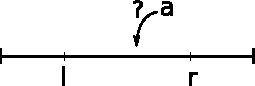
\includegraphics{kap2binsuch}
%  \caption{Ein Beispiel für die Vorgehensweise der Binärsuche.}
%\end{figure}

\begin{Alg}[Binärsuche]
\begin{algorithmic}[1]
\Function{binsuche}{$l$, $r$, $a$}
  \If{$l \le r$}
    \State $k = \frac{l + r}{2}$
    \If{$S[k]==a$}
      \State \textbf{return} $k$
    \ElsIf{$S[k] > a$}
       \State \textbf{return} Binsuche($l$, $k-1$, $a$)
     \Else
       \State \textbf{return} Binsuche($k+1$, $r$, $a$);
    \EndIf
  \Else
    \State \textbf{return} nicht gefunden
  \EndIf
\EndFunction
\end{algorithmic}
\end{Alg}

Betrachten wir die Laufzeit $T(n)$ der Binärsuche, mit $n = |S|$. Der Suchraum wird bei jedem Schritt halbiert. Daher ergibt sich folgende Rekursionsgleichung:
\begin{align*}
  T(1) &= c\\
  T(n) &= T(\lfloor \frac{n}{2} \rfloor) + d
\end{align*}
Daraus folgt $T(n) = \mathcal{O}(\log n)$. Wesentlich effizientere Laufzeit im Mittel weißt die Interpolationssuche auf, die versucht den Suchraum auf den Bereich einzuschränken, in dem ein Treffer erwartet wird.

\subsection{Interpolationssuche}
Nehmen wir an das Universum $\mathcal{U}$ ist ein linear geordnetes Intervall reeller Zahlen, o.B.d.A $\mathcal{U}=[0,1]$. Gehen wir weiter davon aus, dass $S$ unabhängige und gleichverteilte Elemente sind, die zufällig aus $\mathcal{U}$ gewählt wurden.

\begin{Bem}
\hspace{\parindent}Jedes beliebige Intervall lässt sich auf das Intervall $[0,1]$ abbilden und umgekehrt. Aus der Beschränkung folgt lediglich, dass es ein größtes und ein kleinstes Element in $\mathcal{U}$ gibt.\end{Bem}

\begin{figure}[htb]
  \centering
  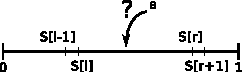
\includegraphics[scale=1.25]{kap2Interpolationssuche}
  \caption{Beispiel: Es soll der Bereich $S[l] \ldots S[r]$ nach $a \in [0,1]$ durchsucht werden, dabei ist $S$ ein aufsteigend sortiertes Feld.}
  \label{interpolationssuche}
\end{figure}

Die Interpolationssuche funktioniert genau wie die Binärsuche, bis auf die Auswahl des Pivotelements $a$. Als Pivotelement wählen wir das $k$-te Element der Folge $S$, wobei $k$ wie folgt definiert ist:
\[ k=l-1 + \left\lceil \frac{a-S[l-1]}{S[r+1]-S[l-1]} \cdot (r-l+1) \right\rceil \]
Wir versuchen also das Element als Pivoelement zu wählen, bei dem wir bei perfekter Gleichverteilung das gesuchte Element erwarten würden.

% 0......S[l-1].S[l]..........S[r].S[r+1]...........1
%           (_________________________)
%                      ^a

%$k=l-1 + \left\lceil \frac{a-S[l-1]}{S[r+1]-S[l-1]} \cdot (r-l+1) \right\rceil$

Möchte man die Rekursionsfolge aufstellen, um die Laufzeit zu berechnen, so sollte man für $S[0] = 0$ und $S[n+1] = 1$ setzen.

Die Laufzeit der Interpolationssuche ist abhängig von der Größe der durchsuchten Folge: $|S|=n$. Im schlechtesten Fall hat die Interpolationssuche eine Laufzeit von $\Theta(n)$, im Mittel liegt die Laufzeit bei $\mathcal{O}(\log\log n)$. Der Beweis der Laufzeit ist zu komplex für diese Veranstaltung.

\subsection{Quadratische Binärsuche}
%           ___ = \sqrt{m}
% ______________________________m   mit m=r-l+1
%...S[l]..||...||...S[k].......S[r]
%                    ^a? sonst
%               ^a? sonst
%          ^a?
Um ein Feldsegment von $S[l]\ldots S[r]$ nach $a \in [0,1]$ zu durchsuchen bestimmen wir das Pivotelement, wie bei der Interpolations-Suche und nennen es $k$. Falls $a=S[k]$ haben wir das gewünschte Element bereits gefunden. Falls $S[k] > a$ überprüfen wir die Elemente $S[k-\sqrt{m}], S[k-2 \sqrt{m}], \ldots , S[k - i \sqrt{m}]$ bis ein Element $\le a$ gefunden wird, wobei $m = r-l+1$. Dann durchsuchen wir rekursiv den Bereich $S[k-i \cdot \lceil\sqrt{m}\rceil] \ldots S[k-(i-1) \cdot \lceil\sqrt{m}\rceil]$. Sollte $a > S[k]$ sein, gehen wir analog vor.

\begin{figure}[hbt]
  \centering
  \includegraphics{kap2quadratischeBinsuche}
  \caption{Quadratische Binärsuche: es wird die erwartete Position von $a$ berechnet. Je nachdem ob der vorgefundene Wert größer oder kleiner ist wird nach links oder rechts um $\sqrt{m}$ Felder gesprungen, bis ein kleinerer/größerer Wert als $a$ gefunden wird. in dem so eingegrenzten Intervall wird dann nach $a$ gesucht.}
  \label{quadratischeBinsuche}
\end{figure}

%$S[k-1\sqrt{m}]$.\\
%durchsuche rekursiv $S[k-i\lceil\sqrt{m}\rceil]...S[k-(i-1) \lceil\sqrt{m}\rceil]$
%Analyse:

\begin{Lza}
\hspace{\parindent}Wie viele Sprünge der Länge $\lceil\sqrt{m}\rceil$ sind im Mittel notwendig um richtiges Intervall der Länge $\lceil\sqrt{m}\rceil$ zu finden? Die Anzahl der Sprünge ist abhängig vom Abstand zwischen der erwarteten Position des gesuchten Elements $a$ und seiner tatsächlichen Position. Die tatsächliche Postion können wir auch mit $rang(a)$ bezeichnen, ihre erwartete Position (den Erwartungswert von $rang(a)$) haben wir mittels $k$ angegeben.

Den Erwartungswert über die der Anzahl der benötigten Sprünge nennen wir $c$. $P_i$ ist die Wahrscheinlichkeit, dass mindestens $i$ Sprünge gebraucht werden um $a$ zu finden. $P_i - P_{i+1}$ entspricht der Wahrscheinlichkeit genau $i$ Sprünge zu brauchen. Wir können dann $c$ berechnen:
\[c = \sum_{i=1}^{\infty} i \cdot (P_i - P_{i+1})\]
Das lässt sich zusammenfassen:
\begin{align*}
  c &= \sum_{i=1}^{\infty} i \cdot (P_i - P_{i+1}) \\
    &= \sum_{i=1}^{\infty} i \cdot P_i - \sum_{j=2}^{\infty} (j-1) \cdot P_{j} \\
    &= P_1 + \sum_{i=2}^{\infty} (i \cdot P_i - (i-1) \cdot P_{i}) \\
    &= \sum_{i=1}^{\infty} P_i %\qquad \text{mit } P_1, P_2 \le 1
\end{align*}

$P_1$ und $P_2$ sind die Wahrscheinlichkeiten, dass mindestens $1$ beziehungsweise mindestens $2$ Sprünge benötigt werden, um $a$ zu finden. Es gilt $P_1, P_2 \le 1$. Bei $i \ge 3$ Sprüngen ist der Rang von $a$ um mindestens $(i-2) \cdot \sqrt{m}$ von seinem Erwartungswert $k$ entfernt, also:
\[ |rang(a) -k| \ge (i-2) \cdot \lceil\sqrt{m}\rceil \]
Also gilt für $i \ge 3$, dass $P_i$ kleiner oder gleich der Wahrscheinlichkeit ist, dass der Abstand zwischen $rang(a)$ und $k$ größer oder gleich $(i-2) \cdot \sqrt{m}$ ist:
\[ P_i \le P(|rang(a) - k| \ge (i-2) \cdot \sqrt{m}) \]

Die Wahrscheinlichkeit, dass der Wert einer Zufallsvariablen sich um mehr als einen gegebenen Wert von dem Erwartungswert dieser Zufallsvariablen unterscheidet, lässt sich mit der Tschebyscheff Ungleichung abschätzen.
\[ P(|X - \mu| \ge t) \le \frac{\sigma^2}{t^2} \]
Dabei ist $X$ die Zufallsvariable und $\mu$ ihr Erwartungswert. $\sigma$ ist die Standardabweichung und $\sigma^2$ ist die Varianz von $X$, das heißt $\sigma^2 (X) = E((X-E(X))^2)$

%$X$ Zufallsvariable und $\mu$ ihr Erwartungswert.
%$\sigma^2$ Varianz von $X = E((X-E(x))^2)$
%$\sigma$ Standardabweichung

\begin{figure}[hbt]
  \centering
  \includegraphics{Suche-Intervall-l_minus_1-r_plus_1}
  \caption{Suche von $a$ über die Teilfolge $S[l] \ldots S[r]$, also über die Werte des Intervalls $\left( S[l-1], S[r+1] \right)$. }
  \label{Suche_Intervall_lr}
\end{figure}

Abbildung \ref{Suche_Intervall_lr} veranschaulicht die Suche von $a$ über der Teilfolge $S[l] \ldots S[r]$, also über die Werte des Intervalls $\left( S[l-1], S[r+1] \right)$. Unsere Zufallsvariable $X(a)$ bildet das gesuchte Element $a$ auf seinen Rang $rang(a)$ ab. Der ist identisch mit der Anzahl der $S[j]$ für die gilt $S[j] \le a$. Wir gehen davon aus, dass $S[j]$ unabhängige, gleichverteilte, gleichmäßig über dem Intervall $(S[l-1], S[r+1])$ gezogene Elemente sind, die nach ihrer Ziehung ihrer Größe nach geordnet wurden. Die Wahrscheinlichkeit, dass ein zufällig aus $(S[l-1], S[r+1])$ gezogenes Element $S[j] \le a$ ist, können wir angeben als
\[ P = \frac{a - S[l-1]}{S[r+1] - S[l-1]} \]
Es ist klar, dass $j = l, \ldots, r$ sein muss. Wir erinnern uns, dass wir $m = r-l+1$ definiert hatten. Nun können wir der Binomialverteilung entsprechend berechnen, wie groß die Wahrscheinlichkeit ist, dass $q$ viele $S[j] \le a$ sind:
\[ \binom{m}{q} \cdot P^q \cdot (1-P)^{m-q} \]

$\binom{m}{q}$ gibt die Möglichkeiten an $q$ Stück aus $m$ auszuwählen. $p^q$ steht für die Wahrscheinlichkeit, dass diese $q$ alle $\le a$ sind. $(1-p)^{q-m}$ entspricht der Wahrscheinlichkeit, dass die restlichen $S[j] >a$ sind.

Der Erwartungswert einer binomialverteilten Größe ist
\begin{align*}
  E(X) &= \mu \\
       &= \sum_{q=0}^{m} q \cdot \binom{m}{q} \cdot P^q \cdot (1-P)^{m-q}\\
       &= P \cdot m
\end{align*}

Ihre Varianz ist
\begin{align*}
  \sigma^2 &= E((X-E(X))^2) \\
           &= E\left(\left(\binom{m}{q} \cdot P^q \cdot (1-q)^{m-q} - P \cdot m\right)^2\right) \\
           &= P \cdot (1-P) \cdot m
\end{align*}

Wir können $P_i$ jetzt durch die Tschebyscheff Ungleichung abschätzen.
\[ \underbrace{P_i}_{\ge i \text{ Sprünge, } i \ge 3} \le \frac{\sigma^2}{t^2} \le \frac{P \cdot (1-P) \cdot m}{((i-2)\sqrt{m})^2} = \frac{P \cdot (1-P)}{(i-2)^2} \]

\begin{figure}[htb]
	\centering
	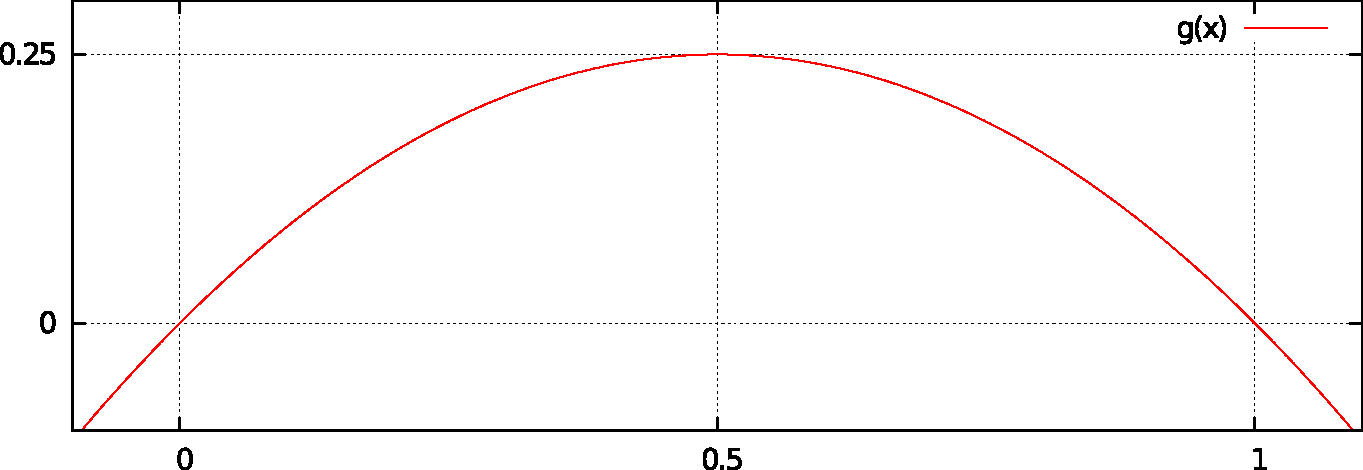
\includegraphics[width=.75 \textwidth]{kap2x-xQuadrat}
	\caption{Visualisierung von $P(1-P)$ zur Abschätzung gegen $0,25$.}
	\label{kap2x-xQuadrat}
\end{figure}

Abbildung \ref{kap2x-xQuadrat} visualisiert $P(1-P)$. Es ist leicht zu sehen, dass wir $P(1-P) \le \frac{1}{4}$ setzen können, also $P_i = \frac{P \cdot (1-P)}{(i-2)^2} \le \frac{1}{4 \cdot (i-2)^2}$.

Nun lässt sich die erwartete Anzahl von Vergleichen genau bestimmen. Weil $P_1, P_2 \le 1$ können wir $P_1+P_2 \le 2$ abschätzen. Dank Gauß wissen wir $\sum_{j=1}^{\infty} \frac{1}{j^2} = \frac{\pi^2}{6}$.

\begin{align*}
	c &= \sum_{i=1}^{\infty} P_i\\
	  &\le 2 + \frac{1}{4} \sum_{i=3}^{\infty} \frac{1}{(i-2)^2} \\
	  &= 2 + \frac{1}{4} \sum_{j=1}^{\infty} \frac{1}{j^2}\\
	  &= 2 + \frac{\pi^2}{24}\\
	  &= 2,411\ldots
\end{align*}

Damit können wir die Rekursionsgleichung für $T(n)$ aufstellen:
\begin{align*}
  T(1) &= b \\
  T(n) &\le T(\sqrt{n}) + c
\end{align*}

$T(\sqrt{n})$ berechnet die Kosten für den rekursiven Aufruf. Den Suchraum kann man im Mittel in konstanter Zeit auf $\sqrt{n}$ einschränken, was durch $c$ (zuvor gegen $2,411\ldots$ abgeschätzt) berücksichtigt wird.

Wir analysieren die Rekursionsgleichung für $n$ der Form $2^{2^k}$.
\begin{align*}
  T(1) &=b \\
  T(n) &\le T(\sqrt{n}) + c \\
       &\le T(n^{\frac{1}{4}}) +2 \cdot c \\
       &\quad\vdots \\
       &\le T(n^{(\frac{1}{2}^a)}) + a \cdot c \\
       &\le T(2) + c \cdot \log \log n
%\\     & = \mathcal{O}(\log \log n)
\end{align*}
$a$ setzen wir also so, dass gilt $n^{\left(\frac{1}{2}^a\right)} = 2$. Daraus folgt:
\begin{align*}
  \log n^{\frac{1}{2^a}} &= 1 \\
  \frac{1}{2^a} \log n &= 1\\
  \log n &= 2^a\\
  \log \log n &= a
\end{align*}
und daher $ T(n) \in \mathcal{O}(\log \log n)$. Für allgemeine $n$ ließe sich durch Induktion zeigen, dass $T(n) \le c \cdot \log \log n$.
\end{Lza}
